\begin{frame}[t]{Data Rate, Bit Rate and Payload Size}
  Overview about \alert{bit rate} and \alert{maximum payload size} with respect to \alert{spreading factor} $SF$ and \alert{bandwidth} $BW$ of a chirp numbered by the \alert{data rate} $DR$:
  \begin{center}
    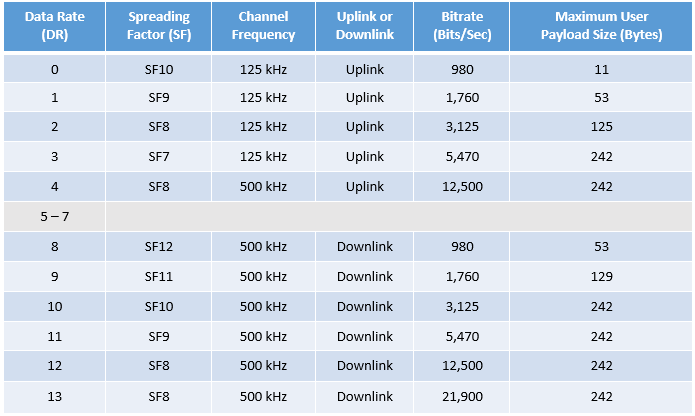
\includegraphics[width=0.45\textwidth]{material/data-rate.png}
  \end{center}
  \begin{description}[$\Rightarrow$]
    \item[$\Rightarrow$] By knowing the configured \alert{data rate} of a device you also know the \alert{bit rate} and maximum \alert{guarantied payload size}.\\
    \item[$\Rightarrow$] The \alert{payload size} can have a \alert{upper limit} if \alert{dwell time} is imposed by the regulator. E.g. US915 a dwell limit of $\SI{400}{\milli\second}$ applies.
  \end{description}
\end{frame}
